Aunque no sea estrictamente necesario, hemos creado un diagrama de Gantt que podemos ver en la figura \ref{fig:gantt1} y \ref{fig:gantt2}, que nos ayude a planificar el tiempo para lograr los objetivos que acabamos de describir.\par
\begin{figure}[ht]
\hspace*{-0.5in}
\centering
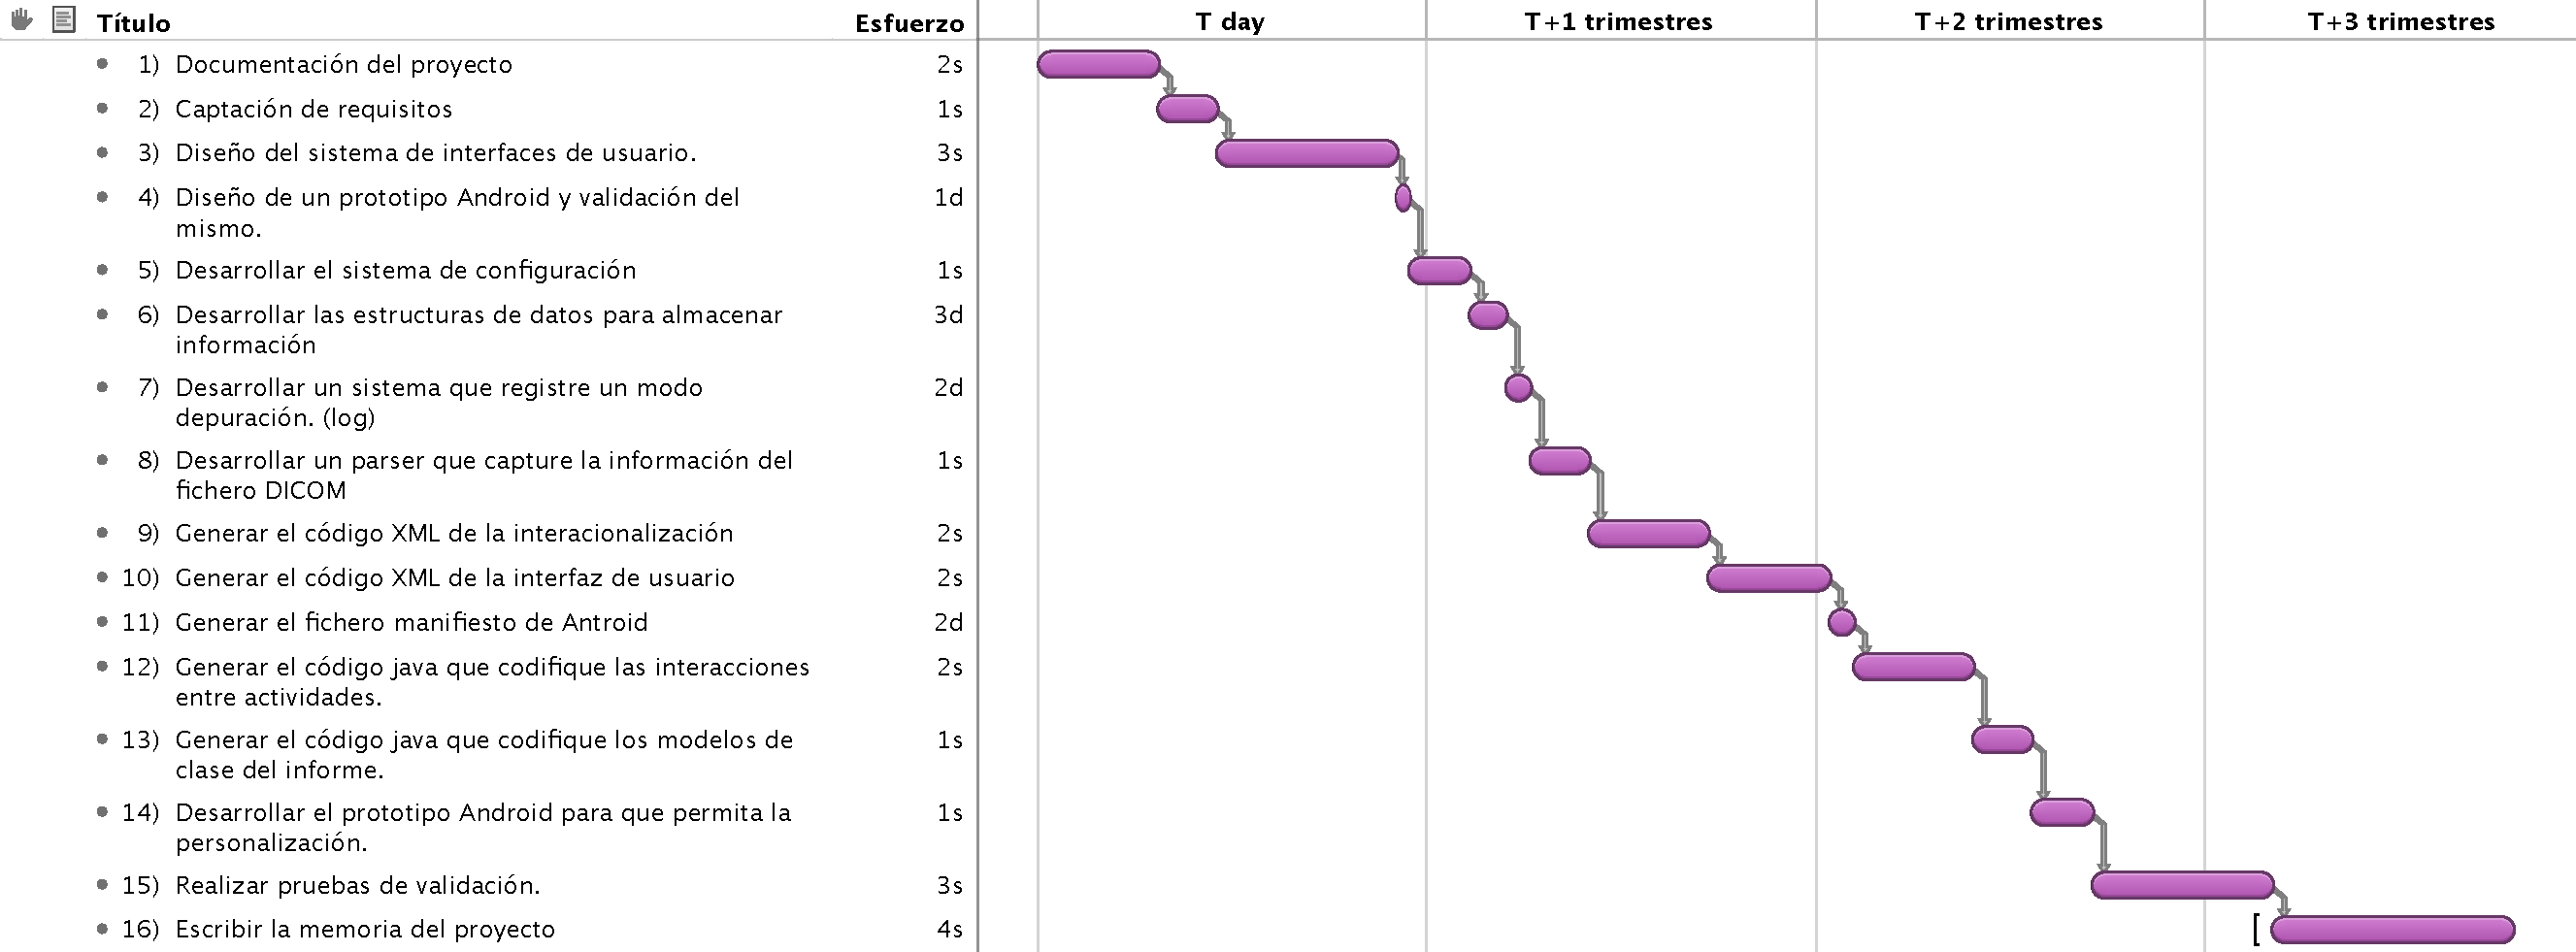
\includegraphics[scale=0.5,  clip, trim=0cm 0cm 12cm 0cm]{./imgs/gantt.pdf}
\caption{Parte 1 del diagrama de Gantt}
\label{fig:gantt1}
\end{figure}
\begin{figure}[ht]
\centering
\hspace*{-1in}
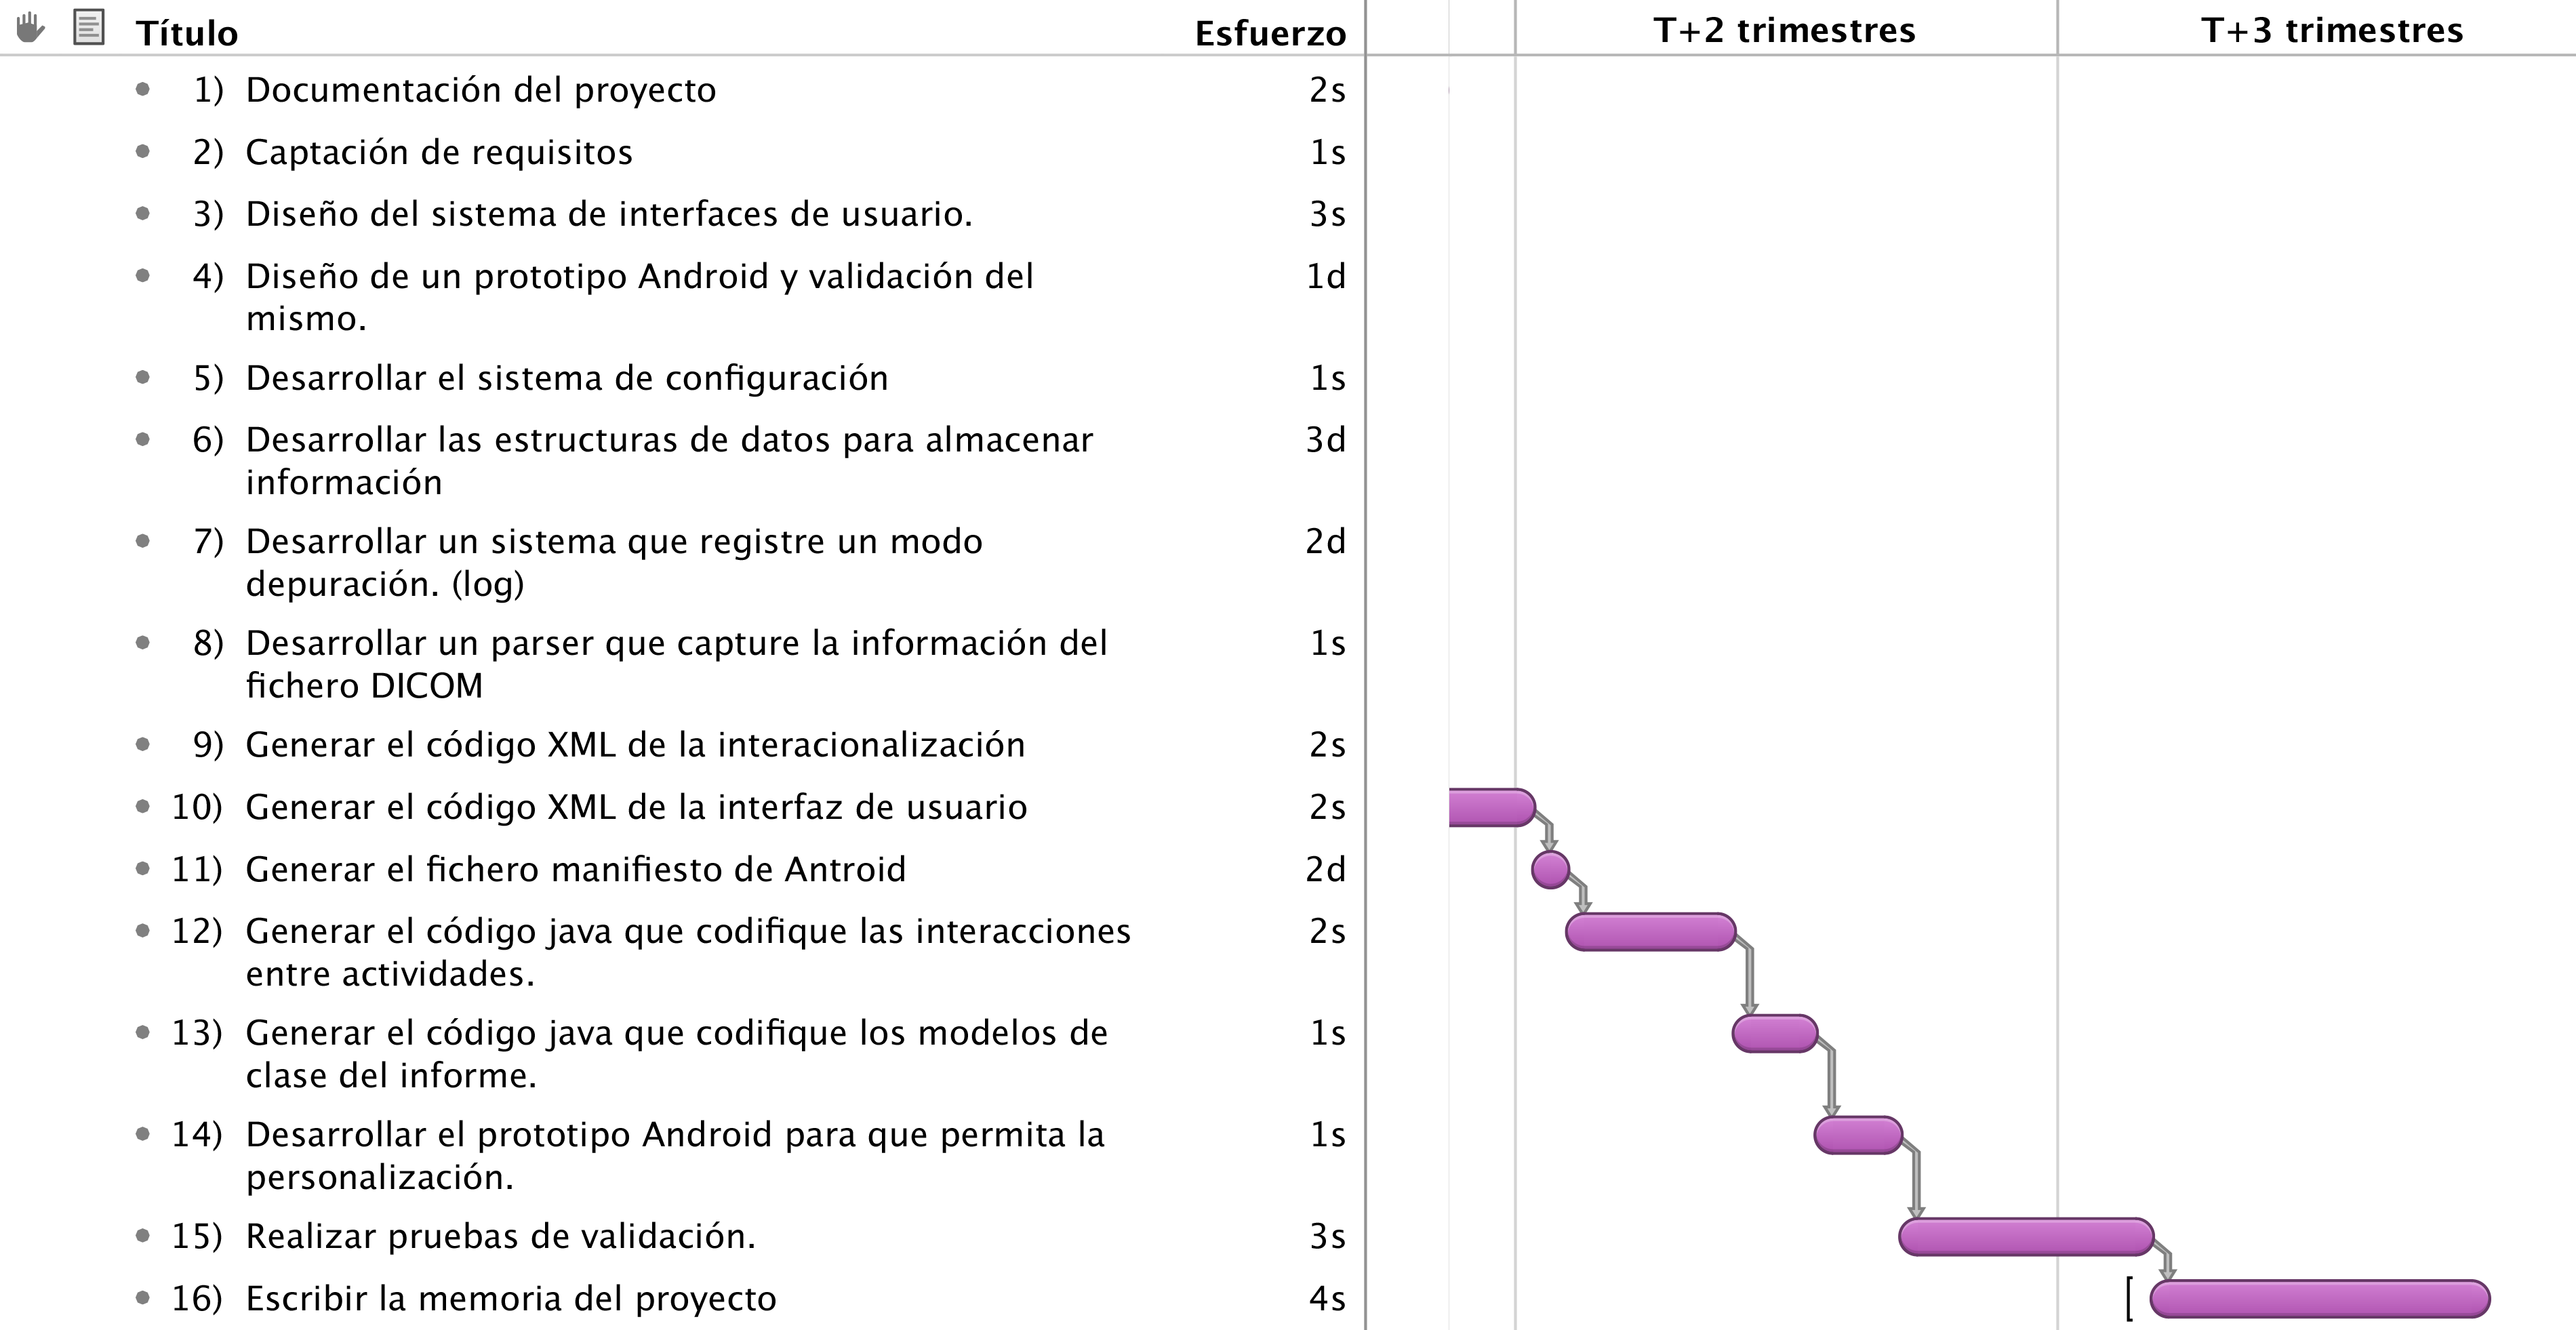
\includegraphics[scale=0.6]{./imgs/planificacion/gantt2.png}
\caption{Parte 2 del diagrama de Gantt}
\label{fig:gantt2}
\end{figure}